\chapter{Specyfikacja zewnętrzna}
\label{ch:04}

Aplikacja została stworzona w środowisku Unity i zapewnia interaktywną symulację rozprzestrzeniania się zarażeń w przestrzeni biurowej. Pozwala na zmianę wielu parametrów wpływających na przebieg symulacji. Ma na celu w prosty i zrozumiały dla każdego sposób pokazywać rozprzestrzenianie się choroby. Przeznaczona jest głównie dla użytkowników korzystających z komputerów osobistych z systemem operacyjnym Windows.

\section{Wymagania}

Sprzęt i oprogramowanie potrzebne do uruchomienia aplikacji:
\begin{itemize}
	\item Komputer z systemem operacyjnym Windows.
	\item Ekran o rozdzielczości co najmniej 1280x720 pikseli.
	\item Karta graficzna wspierająca OpenGL 3.2 lub nowszy.
	\item System operacyjny: Windows 7/8/10 i nowsze.
	\item Zainstalowany runtime Unity w wersji zgodnej z aplikacją.
\end{itemize}

\section{Uruchamianie aplikacji}

Aby skorzystać z aplikacji, należy wykonać poniższe kroki:

\begin{enumerate}
	\item Pobrać folder zawierający aplikację.
	\item Rozpakować pobrany folder w wybranym miejscu na dysku.
	\item Kliknąć w folder aplikacji.
	\item Kliknąć dwukrotnie plik wykonywalny \textit{exe} aplikacji.
\end{enumerate}

Aplikacja uruchomi się bez konieczności instalacji.

\section{Obsługa aplikacji}

Do obsługi aplikacji wystarczy myszka, która umożliwia interakcję z interfejsem graficznym. Aplikacja nie wymaga dodatkowego sprzętu.
\begin{itemize}
	\item \textbf{Ustawianie Parametrów Symulacji}
	
	Dostosowywanie parametrów odbywa się poprzez ustawianie suwaków znajdujących się z prawej strony (widocznych na rysunku \ref{fig:beforeSim} przy numerze pierwszym) za pomocą myszki. Parametry należy ustawić przed rozpoczęciem symulacji, ich zmiana w jej trakcie nie wpłynie na jej przebieg, a nowe ustawienia zostaną wprowadzone dopiero po restarcie symulacji. Wyjątkiem jest prędkość symulacji którą można zmieniać w trakcie działania programu.\\
	\textbf{Lista dostępnych parametrów:}
	\begin{itemize}
		\item \textbf{Dystans zarażenia:}\\
		 Dystans przenoszenia się wirusa.
		
		\item \textbf{Czas do zarażenia:}\\
		 Długość bliskiego kontaktu z chorym,aby doszło do zarażenia.

		\item \textbf{Zaraźliwość patogenu:}\\
		 Zdolność wirusa do zarażania.
		
		\item \textbf{Średni okres inkubacji:}\\
		Czas od narażenia do rozwinięcia się objawów.

		\item \textbf{Procent populacji noszący maseczki:}\\
		Procentowa ilość ludzi noszących maseczki.

		\item \textbf{Skuteczność maseczek:}\\
		Określa jak bardzo skuteczne są maseczki w ograniczaniu zasięgu wirusa.
		
		\item \textbf{Liczebność populacji:}\\
		Ogólna liczba postaci uczestniczących w symulacji.
		
		\item \textbf{Początkowy procent zarażonych:}\\
		Procentowej liczba zarażonych na początku symulacji.
		
		\item \textbf{Odporność populacji:}\\
		Odporności osobników na zarażenie.

		\item \textbf{Długość symulacji:}\\
		Ilość dni trwania symulacji.
		
		\item \textbf{Prędkość symulacji:}\\
		Umożliwienie regulacji prędkości symulacji, włączając przyspieszenie do 100-krotności normalnej prędkości.
		
		\item \textbf{Średni czas wykrycia:}\\
		Czas jaki upływa od momentu pojawienia się objawów do ich wykrycia i zlecenia kwarantanny.
	\end{itemize}
	
	\item \textbf{Rozpoczęcie symulacji i jej kontrola}\\
	Do kontroli symulacji służą przyciski widoczne na rysunku \ref{fig:beforeSim} przy numerze drugim. Są to \textit{Start},\textit{Pauza} i \textit{Restart}. 
	
	\begin{itemize}
	\item \textbf{Start}\\
	Uruchamia symulację lub ją wznawia.
	
	\item \textbf{Pauza}\\
	Zatrzymuje symulacje. Po jej wznowieniu parametry symulacji, pozycje agentów i czas się nie zmieniają.
	
	\item \textbf{Restart}\\
	Kończy symulację. Usuwa wszystkich agentów, po uruchomieniu symulacji agenci zostaną stworzeni na nowo wraz ze zaktualizowanymi parametrami.
	\end{itemize}
	
	\item \textbf{Zakończenie symulacji}\\
	Użytkownik może zakończyć symulację w każdej chwili klikając w przycisk \textit{Restart}. W przeciwnym przypadku symulacja zakończy się automatycznie po ustawionym na początku czasie jej trwania oraz zostanie wyświetlony ekran z podsumowaniem widoczny na rysunku \ref{fig:endSim}.
	
	\item \textbf{Statystyki symulacji}\\
	Podczas trwania symulacji możliwe jest bieżące monitorowanie jej statystyk co widać na rysunku \ref{fig:beforeSim} przy numerze trzecim. Sa to liczba osób narażonych, liczba zarażonych, aktualny czas w środowisku symulacyjnym oraz rzeczywisty czas od rozpoczęcia.
\end{itemize}

\begin{figure}[h!]
	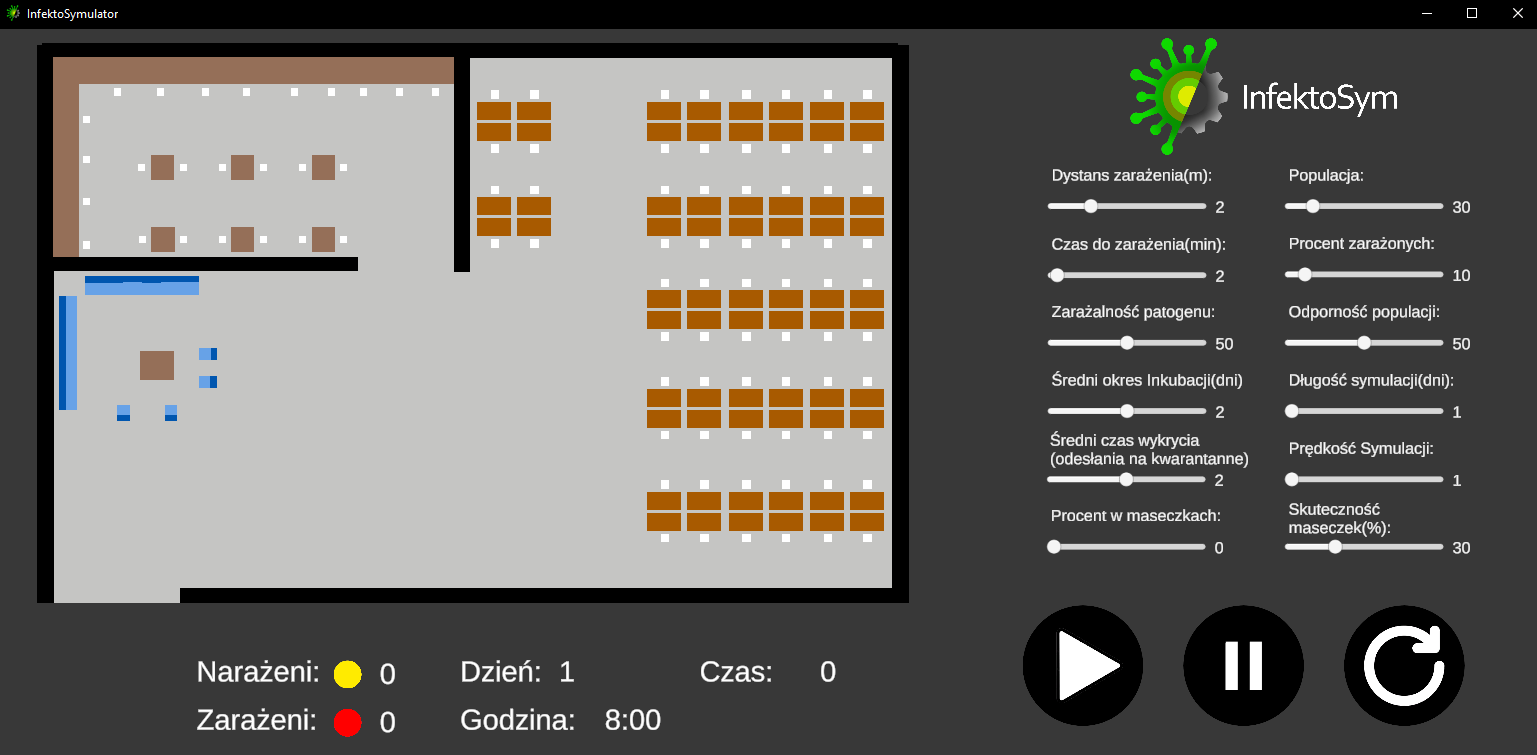
\includegraphics[width=\linewidth]{beforeSim.png}
	\caption{Ekran początkowy aplikacji.}
	\label{fig:beforeSim}
\end{figure}

\begin{figure}[h!]
	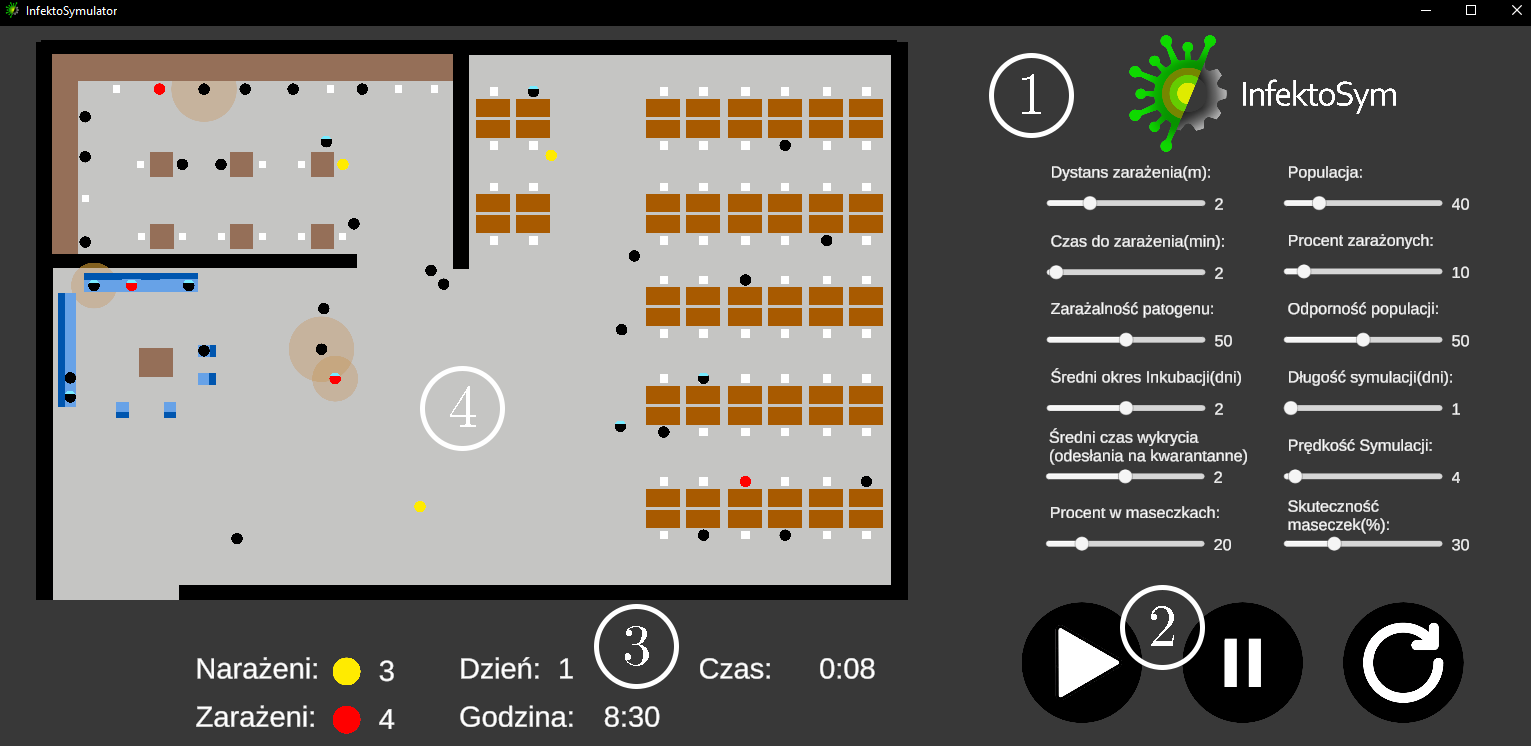
\includegraphics[width=\linewidth]{runningSimwithNumbers.png}
	\caption{Ekran podczas działającej symulacji: 1. Suwaki do ustawiania parametrów, 2. Przyciski kontrolujące 3. Aktualne statystyki i czas, 4. Wizualizacja}
	\label{fig:runningSim}
\end{figure}

\begin{figure}[h!]
	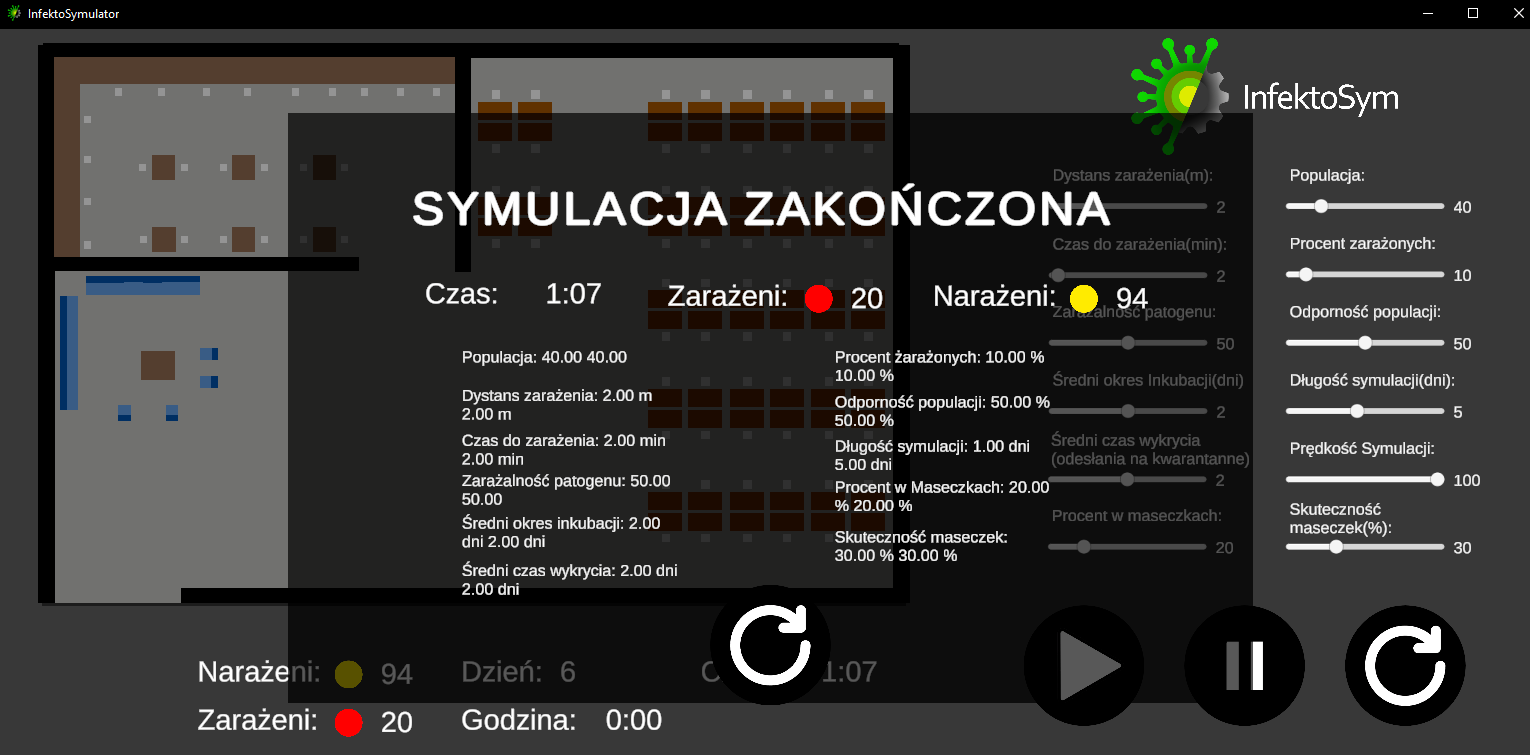
\includegraphics[width=\linewidth]{endSim.png}
	\caption{Ekran zakończenia symulacji}
	\label{fig:endSim}
\end{figure}

\begin{figure}[h!]
	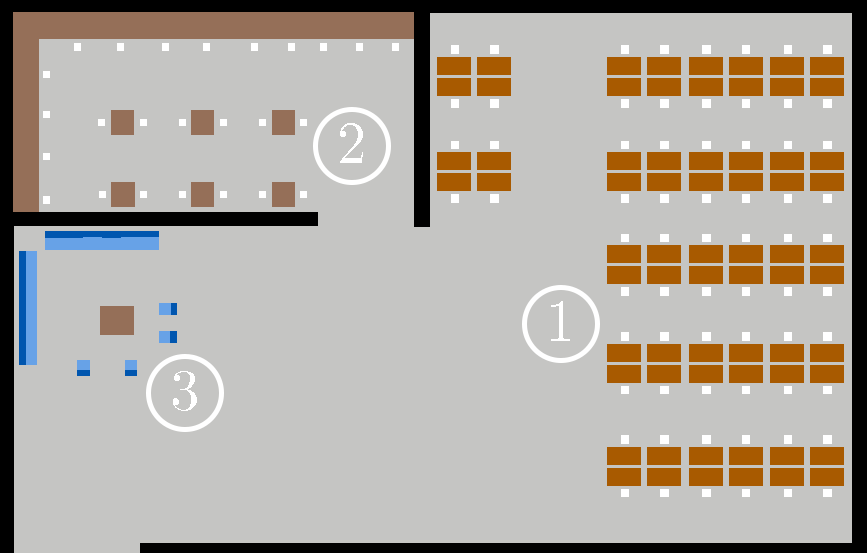
\includegraphics[width=\linewidth]{mapWithNumbers.png}
	\caption{Mapa biura: 1. Biurka do pracy, 2. Kuchnia ze stolikami, 3. Miejsce wypoczynku}
	\label{fig:simMap}
\end{figure}


%%%%%%%%%%%%%%%%%%%%%
%% RYSUNEK Z PLIKU
%
%\begin{figure}
%\centering
%
\includegraphics[width=0.5\textwidth]{./graf/politechnika_sl_logo_bw_pion_pl.pdf}
%\caption{Podpis rysunku zawsze pod rysunkiem.}
%\label{fig:etykieta-rysunku}
%\end{figure}
%Rys. \ref{fig:etykieta-rysunku} przestawia …
%%%%%%%%%%%%%%%%%%%%%
%
%%%%%%%%%%%%%%%%%%%%%
%% WIELE RYSUNKÓW 
%
%\begin{figure}
%\centering
%\begin{subfigure}{0.4\textwidth}
%    
\includegraphics[width=\textwidth]{./graf/politechnika_sl_logo_bw_pion_pl.pdf}
%    \caption{Lewy górny rysunek.}
%    \label{fig:lewy-gorny}
%\end{subfigure}
%\hfill
%\begin{subfigure}{0.4\textwidth}
%    
\includegraphics[width=\textwidth]{./graf/politechnika_sl_logo_bw_pion_pl.pdf}
%    \caption{Prawy górny rysunek.}
%    \label{fig:prawy-gorny}
%\end{subfigure}
%
%\begin{subfigure}{0.4\textwidth}
%    
\includegraphics[width=\textwidth]{./graf/politechnika_sl_logo_bw_pion_pl.pdf}
%    \caption{Lewy dolny rysunek.}
%    \label{fig:lewy-dolny}
%\end{subfigure}
%\hfill
%\begin{subfigure}{0.4\textwidth}
%    
\includegraphics[width=\textwidth]{./graf/politechnika_sl_logo_bw_pion_pl.pdf}
%    \caption{Prawy dolny rysunek.}
%    \label{fig:prawy-dolny}
%\end{subfigure}
%        
%\caption{Wspólny podpis kilku rysunków.}
%\label{fig:wiele-rysunkow}
%\end{figure}
%Rys. \ref{fig:wiele-rysunkow} przestawia wiele ważnych informacji, np. rys. \ref{fig:prawy-gorny} jest na prawo u góry.
%%%%%%%%%%%%%%%%%%%%%


